\documentclass[12pt]{extarticle}
\usepackage[utf8]{inputenc}
\usepackage{cite}
\usepackage{graphicx}

\title{ODE Solver Design Report}
\author{
  Mahmoud Adas\\
  \texttt{Section:2, BN:21}
  \and
  Evram Youssef\\
  \texttt{Section:1, BN:9}
  \and
  Remonda Talaat\\
  \texttt{Section:1, BN:20}
  \and
  Mohamed Shawky\\
  \texttt{Section:2, BN:16}
}

\begin{document}

\maketitle

 \begin{figure}[hp]
    \centering
    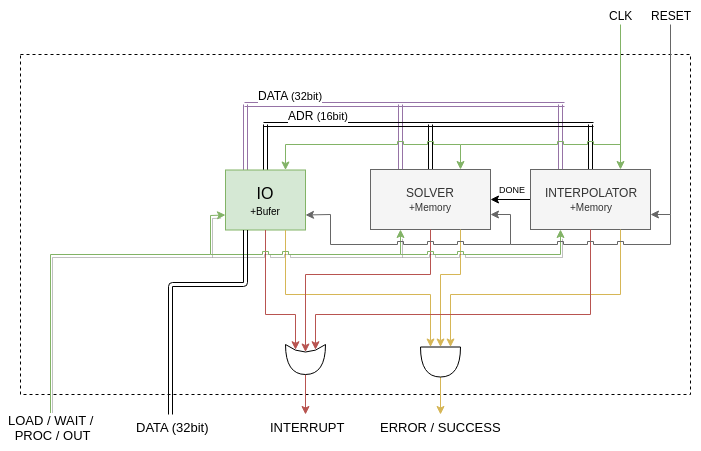
\includegraphics[width=\textwidth]{d1}
    \caption{Overall Design}
    \label{fig:overall}
\end{figure}

\section{Variables Specs}
\begin{itemize}
    \item N : 6 bits [1:50]
    \item M : 6 bits [1:50]
    \item C : 3 bits [1:5]
    \item h : 64 bits
    \item err : 64 bits
    \item mode : 1 bit [0,1]
    \item fp: 2 bits [0,1,2]
    \item A : 160000 bits, [N*N] each number could be 16bit fixed point/ floating point 32/ or floating point 64
    \item B : 160000 bits, [N*M] each number could be 16bit fixed point/ floating point 32/ or floating point 64
    \item X : 3200 bits, [N*1] each number....
    \item U : 3200 bits, [M*1] each number....
    \item T\_s : 320 bits, [5*1] each number....
    \item X\_out : 16000 bits [N*1]*5
\end{itemize}


\section{Interfaces and HW Summary}
The hardware has the following interfaces that triggers some actions summarized below and detailed in the rest of the document.
\begin{itemize}
    \item CLK: IN
    \item RESET: ASYNC IN
    \begin{itemize}
        \item clears all internal states of all modules:
        \begin{itemize}
            \item IO internal buffer.
            \item ERROR/SUCCESS of all modules resets to SUCCESS.
            \item INTERRUPT resets to zero.
        \end{itemize}
        \item Memory at solver and interpolator are NOT cleared.
        \item at next clock, CPU is expected to turn the \emph{LOAD / WAIT / PROC / OUT} into \emph{LOAD} state and we will start loading input again.
    \end{itemize}
    \item LOAD / WAIT / PROC / OUT (2bit): IN:
    \begin{itemize}
        \item set the current major state of the machine
        \item LOAD(0):
        \begin{itemize}
            \item IO receives \textbf{compressed} data from the CPU.
            \item IO decompresses data into buffer.
            \item buffer is flushed into data bus with appropriate address.
            \item ends when cpu finishes its data loading and switches to \emph{WAIT} state.
        \end{itemize}
        \item WAIT(1):
        \begin{itemize}
            \item Same state as \emph{LOAD}, but IO doesn't receive anymore data from CPU.
            \item ends when IO flushes all its buffer and raises \emph{INTERRUP} with either \emph{ERROR} or \emph{SUCCESS}.
        \end{itemize}
        \item PROC(2):
        \begin{itemize}
            \item SOLVER sends time step to calculate \emph{U} at.
            \item SOLVER and INTERPOLATOR work concurrently to calculate their outputs.
            \item INTERPOLATOR sends \emph{DONE} signal to SOLVER when it finishes the interpolated U.
            \item SOLVER can request to copy the interpolated \emph{U}.
            \item INTERPOLATOR waits for SOLVER to send next time step.
            \item ends when either SOLVER or INTERP raises INTERRUPT with either \emph{SUCCESS} or \emph{ERROR}.
        \end{itemize}
        \item OUT(3):
        \begin{itemize}
            \item IO just copies final outputs to cpu from SOLVER memory.
            \item ends when IO raises INTERRUPT with either \emph{SUCCESS} or \emph{ERROR}.
        \end{itemize}
    \end{itemize}
    \item DATA (32bit): INOUT
    \begin{itemize}
        \item Data bus between cpu and io.
    \end{itemize}
    \item INTERRUPT: OUT
    \begin{itemize}
        \item raised from 0 to 1 when some internal module (IO / SOLVER / INTERPOLATOR) finishes its task.
        \item if task finished with success the \emph{ERROR / SUCCESS} is set to \emph{SUCCESS}, otherwise it's \emph{ERROR}.
    \end{itemize}
    \item ERROR(0) / SUCCESS(1): OUT
    \begin{itemize}
        \item CPU should operate on this value ONLY when \emph{INTERRUPT} is 1.
        \item errors that could happen include: divide by zero, H > 1, incomplete input.
    \end{itemize}
\end{itemize}


\section{Simulation Workflow}

\subsection{Input Preparing}
This stage is the responsibility of a script that runs before the simulation:
\begin{itemize}
    \item INPUT: json file that follows the format stated in main document.
    \item create bit stream of the read data that follows the \emph{Input Data Structure} specifications.
    \item encode the bits following the \emph{Compression} specifications.
    \item collect encoding output in ASCII string, each byte in string is either '0' or '1' in ASCII format.
    \item when the string reaches the length of 32 bytes, push it to output file.
    \item if the last created string didn't reach the length of 32 bytes, complete the rest with '0' and push it to the output file.
    \item OUTPUT:
    \begin{itemize}
        \item ASCII file that contains multiple lines of compressed data.
        \item each line has exactly 32 '0' or '1' ASCII characters.
        \item ONLY the ASCII characters 0 or 1 are permitted in the file and NOTHING ELSE.
        \item there is NO EMPTY LINE/s in the file or spaces.
    \end{itemize}
\end{itemize}

\subsection{Instantiating HW}
This stage and all the next ones are the responsibility of the CPU simulation code.

CPU is a non-synthesisable HDL test-bench that:
\begin{itemize}
    \item instantiates the HW main module.
    \item attaches the appropriate signals to the HW main module.
    \item generates CLK with fixed frequency.
    \item loads data into HW.
    \item puts HW into PROCESS state.
    \item load output out from the HW and into a file.
\end{itemize}

\subsection{Loading Input}
\begin{itemize}
    \item load the output of the former script into array of vectors each is 32bit wide that will hold one line in the file.
    \item put HW at LOAD state.
    \item RESET for one cycle.
    \item for each 32bit vector in the former array:
    \begin{itemize}
        \item at the positive edge of CLK:
        \begin{itemize}
            \item load vector into \emph{DATA} bus.
        \end{itemize}
    \end{itemize}
    \item load DATA with 0s.
    \item wait for the positive edge of \emph{INTERRUPT} signal.
    \item check for \emph{ERROR / SUCCESS} and only proceed if it is SUCCESS.
\end{itemize}

\subsection{Processing}
\begin{itemize}
    \item put HW at PROCESS state.
    \item wait for the \emph{INTERRUPT} positive edge.
    \item check for \emph{ERROR / SUCCESS} and only proceed if it is SUCCESS.
\end{itemize}

\subsection{Extracting Output}
\begin{itemize}
    \item put high impedance on \emph{DATA} bus.
    \item put HW at OUT state.
    \item keep receiving data into array of vectors and outputting them into file in the same format of the input file.
    \item wait for the positive edge of \emph{INTERRUPT} signal. 
\end{itemize}
Simulation is done! 

You can turn the output into human-readable json using output-formatting script.
    
\end{document}

